\documentclass[a4paper, fontsize=11pt]{scrartcl} % A4 paper and 11pt font 
\usepackage[a4paper,left=3cm,right=2cm,top=2.5cm,bottom=2.5cm]{geometry}

\usepackage[T1]{fontenc} % Use 8-bit encoding that has 256 glyphs
\usepackage{fourier} % Use the Adobe Utopia font for the document - comment this line to return to the LaTeX default
\usepackage[spanish]{babel} % Spanish language/hyphenation
\selectlanguage{spanish}
\usepackage[utf8]{inputenc}
\usepackage{amsmath,amsfonts,amsthm} % Math packages
\usepackage{graphicx} % The graphicx package
\usepackage{placeins}
\usepackage{caption}
\usepackage{subcaption}


\usepackage{listings} % Insert Scripts
\usepackage{color} %red, green, blue, yellow, cyan, magenta, black, white
\definecolor{mygreen}{RGB}{28,172,0} % color values Red, Green, Blue
\definecolor{mylilas}{RGB}{170,55,241}

\lstset{language=Matlab,%
	%basicstyle=\color{red},
	breaklines=true,%
	morekeywords={matlab2tikz},
	keywordstyle=\color{blue},%
	morekeywords=[2]{1}, keywordstyle=[2]{\color{black}},
	identifierstyle=\color{black},%
	stringstyle=\color{mylilas},
	commentstyle=\color{mygreen},%
	showstringspaces=false,%without this there will be a symbol in the places where there is a space
	numbers=left,%
	numberstyle={\tiny \color{black}},% size of the numbers
	numbersep=9pt, % this defines how far the numbers are from the text
	emph=[1]{for,end,break},emphstyle=[1]\color{red}, %some words to emphasise
	%emph=[2]{word1,word2}, emphstyle=[2]{style},    
}

\usepackage{sectsty} % Allows customizing section commands
%\allsectionsfont{\centering \normalfont\scshape} % Make all sections centered, the default font and small caps

\usepackage{fancyhdr} % Custom headers and footers
\pagestyle{fancyplain} % Makes all pages in the document conform to the custom headers and footers
\fancyhead{} % No page header - if you want one, create it in the same way as the footers below
\fancyfoot[L]{} % Empty left footer
\fancyfoot[C]{} % Empty center footer
\fancyfoot[R]{\thepage} % Page numbering for right footer
\renewcommand{\headrulewidth}{0pt} % Remove header underlines
\renewcommand{\footrulewidth}{0pt} % Remove footer underlines
\setlength{\headheight}{13.6pt} % Customize the height of the header

\numberwithin{equation}{section} % Number equations within sections (i.e. 1.1, 1.2, 2.1, 2.2 instead of 1, 2, 3, 4)
\numberwithin{figure}{section} % Number figures within sections (i.e. 1.1, 1.2, 2.1, 2.2 instead of 1, 2, 3, 4)
\numberwithin{table}{section} % Number tables within sections (i.e. 1.1, 1.2, 2.1, 2.2 instead of 1, 2, 3, 4)

%\setlength\parindent{0pt} % Removes all indentation from paragraphs - comment this line for an assignment with lots of text

\newenvironment{myalign}{\par\nobreak\large\noindent\align}{\endalign} %Altering fontsize in equations globally

%----------------------------------------------------------------------------------------
%	TITLE SECTION
%----------------------------------------------------------------------------------------

\newcommand{\horrule}[1]{\rule{\linewidth}{#1}} % Create horizontal rule command with 1 argument of height

\title{	
	\normalfont \normalsize 
	\textsc{Master en Automática y Robótica - UPM} \\ [25pt] % Your university, school and/or department name(s)
	\horrule{0.5pt} \\[0.4cm] % Thin top horizontal rule
	\huge Identificación de Función de Transferencia \\ % The assignment title
	\horrule{2pt} \\[0.5cm] % Thick bottom horizontal rule
}

\author{Jorge Camarero Vera - 07052} % Your name

\date{\normalsize\today} % Today's date or a custom date

\begin{document}
	\maketitle
	
	\section{Explicación de la tarea}
	
	Calcular la función de transferencia que contiene el bloque \textit{sistema lineal1} en el archivo \textit{sistema\_tema\_3y4}. 
	
	\begin{figure}[h!]
		\centering
		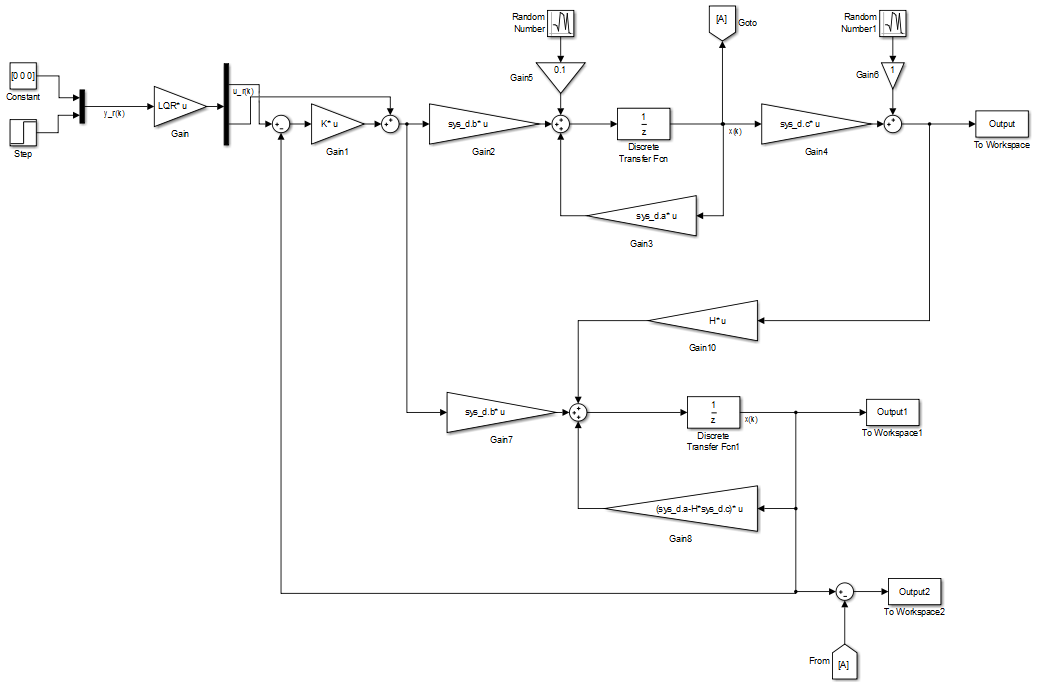
\includegraphics[width=1.0\linewidth]{images/model.JPG}
		\caption{Modelo inicial}
		\label{Modelo Inicial}
	\end{figure}
	\FloatBarrier
	
	\subsection{Presentación de los datos}
	
	Los valores de los pulsos de entrada son los de la Figura \ref{Entrada} y los de la salida los de la Figura \ref{Salida con ruido}, esta salida tiene un ruido añadido con media en 0 y varianza de 0.6.
	
	\begin{figure}[h!]
		\centering
		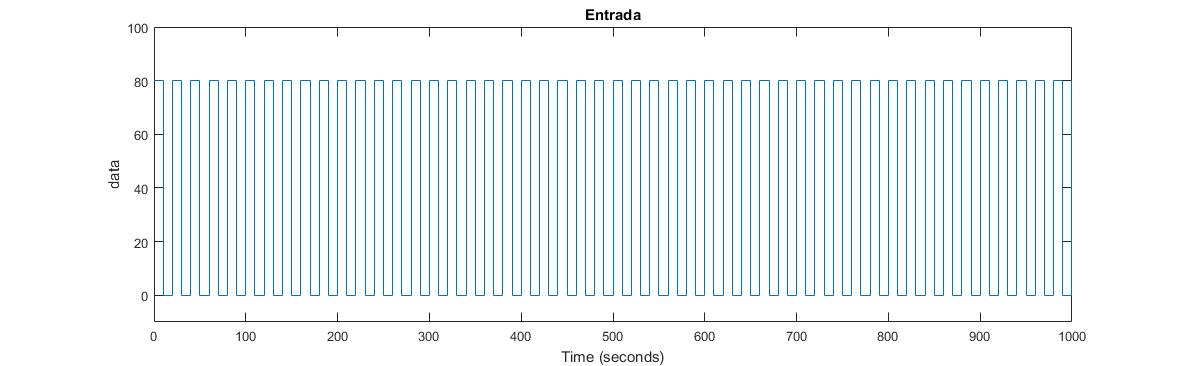
\includegraphics[width=1.0\linewidth]{images/input.PNG}
		\caption{Entrada}
		\label{Entrada}
	\end{figure}
	\FloatBarrier
	
	\begin{figure}[h!]
		\centering
		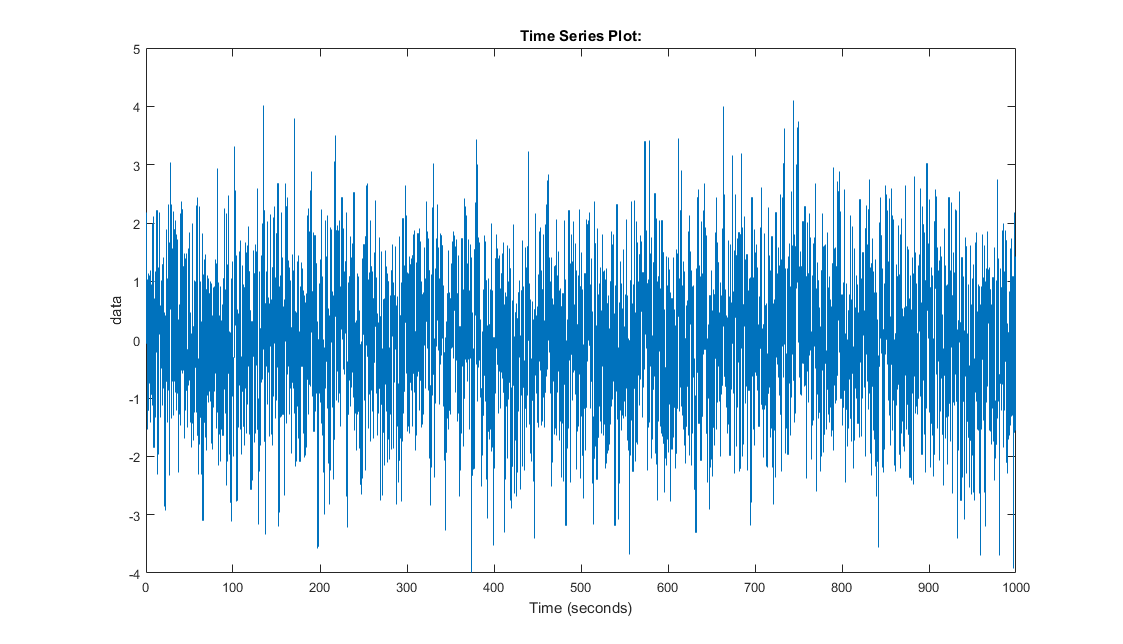
\includegraphics[width=1.0\linewidth]{images/output.PNG}
		\caption{Salida con ruido}
		\label{Salida con ruido}
	\end{figure}
	\FloatBarrier
	
	A partir de estos datos habrá que obtener la función de transferencia. Vamos a estudiar primero el caso sin ruido y después el que tiene ruido.

	\section{Identificación de la Función de Transferencia}	
	
	La función de transferencia a identificar tiene la forma,
	
	\begin{myalign}
		H(z)=\dfrac{b_0+b_1z^{-1}+\cdots+b_mz^{-m}}{1+a_1z^{-1}+\cdots+a_nz^{-n}}
		\label{Transfer Function}
	\end{myalign}
	
	Para identificarla se emplea el método de mínimos cuadrados, el cuál se emplea para la identificación de Sistemas Discretos, estimando los parámetros que mejor se ajustan.
	
	\begin{myalign}		
		y_k+a_1y_{k-1}+a_2y_{k-2}+\cdots+a_ny_{k-n} = b_1u_{k-1}+b_2u_{k-2}+\cdots+b_1u_{k-m}
	\end{myalign}
	
	Si se expresa el error de modelado como:
	
	\begin{myalign}
		\begin{split}
		\epsilon_k &= y_k+a_1y_{k-1}+a_2y_{k-2}+\cdots+a_ny_{k-n}\\
				   &-b_1u_{k-1}-b_2u_{k-2}-\cdots-b_1u_{k-m}
		\end{split}
	\end{myalign}
	
	Teniendo como objetivo determinar los valores de los parámetros:
	
	\begin{myalign}
		\theta = [a_1 a_2 ... a_n b_0 b_1 ... b_m]
	\end{myalign}
	
	Este vector $\theta$ tiene que minimizar el índice cuadrático del error,  $E_c=\sum_{k=1}^{N}\epsilon_k^2$\\
	
	Los datos hay que agruparlos de la siguiente forma:
	
	
	\[ \left[ \begin{array}{c}
	\epsilon_1 \\
	\epsilon_2 \\
	\vdots	   \\
	\epsilon_N 
	\end{array} \right] = \left[ \begin{array}{c}
	y_{1} \\
	y_{1} \\
	\vdots \\
	y_{N} 
	\end{array} \right] - \left[ \begin{array}{cccccccc}
	-y_{0} & -y_{-1} & \cdots & -y_{1-n} & u_0 & u_{-1} & \cdots & u_{1-m} \\
	-y_{1} & -y_{0} & \cdots & -y_{2-n} & u_1 & u_{0} & \cdots & u_{2-m} \\
	\vdots & \vdots & \vdots & \vdots & \vdots & \vdots & \vdots & \vdots \\
	-y_{N-1} & -y_{N-2} & \cdots & -y_{N-n} & u_{N-1} & u_{N-2} & \cdots & u_{N-m} 
	\end{array} \right] \cdot \left[ \begin{array}{c}
	a_1 \\
	a_2 \\
	\vdots \\
	a_n \\
	b_1 \\
	b_2 \\
	\vdots \\
	b_m 
	\end{array} \right]\] 
	
	De forma simplificada:
	
	\begin{myalign}
		\epsilon = y -\Phi \cdot \theta
	\end{myalign}
	
	Finalmente lo que se busca es resolver la siguiente ecuación:
	
	\begin{myalign}
		\hat{\theta}_N = \left[ \Phi^t \cdot \Phi \right]^{-1} \cdot \Phi^t \cdot y
	\end{myalign}
	
	
	Para el cálculo de mínimos cuadrados se ha creado una clase \textit{Caract\_ZTransfor.m}, la cuál al final de este documento se detallará. Se inicializa introduciendo el vector con los datos de la entrada y el vector con los datos de la salida. La función para el cálculo de mínimos cuadrados se deberá pasar los valores de $n$ y $m$ deseados.
		
	\subsection{Sistema sin Ruido}
	
	Al sistema planteado se le quita el ruido, quedando la Figura \ref{Modelo sin ruido}, y la salida la Figura \ref{Salida sin ruido}.
	
	\begin{figure}[h!]
		\centering
		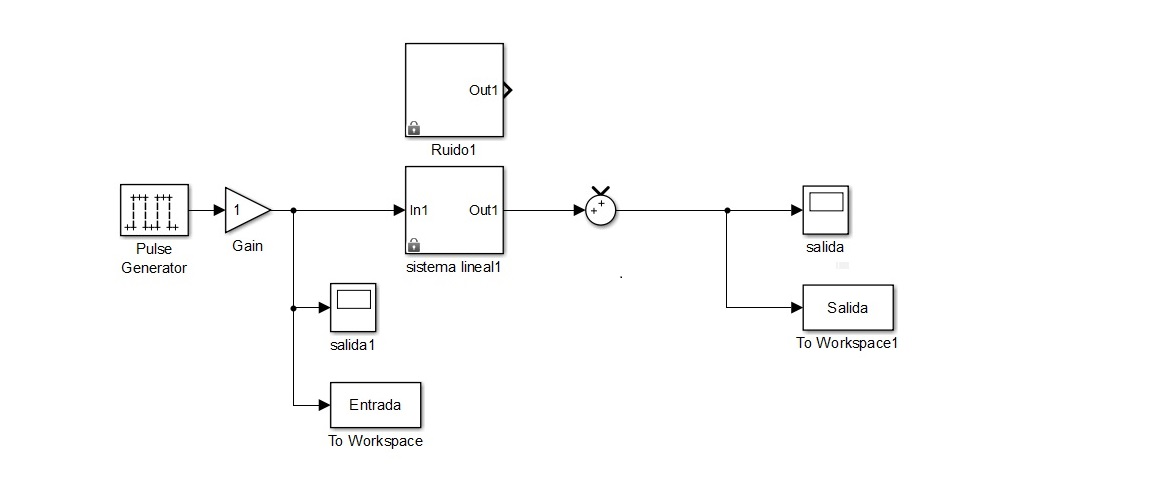
\includegraphics[width=1.0\linewidth]{images/modelNoise.JPG}
		\caption{Modelo sin ruido}
		\label{Modelo sin ruido}
	\end{figure}
	\FloatBarrier
	
	\begin{figure}[h!]
		\centering
		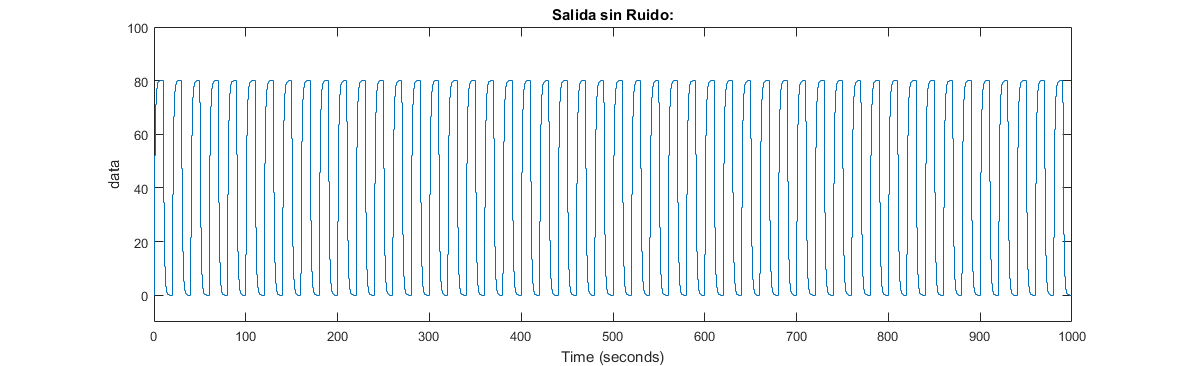
\includegraphics[width=1.0\linewidth]{images/outputNoise.PNG}
		\caption{Salida sin ruido}
		\label{Salida sin ruido}
	\end{figure}
	\FloatBarrier
	
	Se realiza el cálculo de mínimos cuadrados:
	
	\begin{lstlisting}
	>> Zeta = Caract_ZTransform(Entrada.Data,Salida.Data);
	>> theta = Zeta.LeastSquares(1,1)
	
	theta =
	
	-0.9000
	 0.1000
	\end{lstlisting}
	
	
	Entonces siguiendo la fórmula \ref{Transfer Function}, $-0.9$ corresponde a $a_1$ y $0.1$ corresponde a $b_0$, quedando:
	
	\begin{myalign}
			H(z^{-1})= \dfrac{0.1}{1 - 0.9z^{-1}}
			\label{TF Identify}
	\end{myalign}
	
	Comprobamos en el modelo Figura \ref{Modelo Filtro} y obtenemos las salida Figura \ref{Comparativa}. 
	
	\begin{figure}[h!]
		\centering
		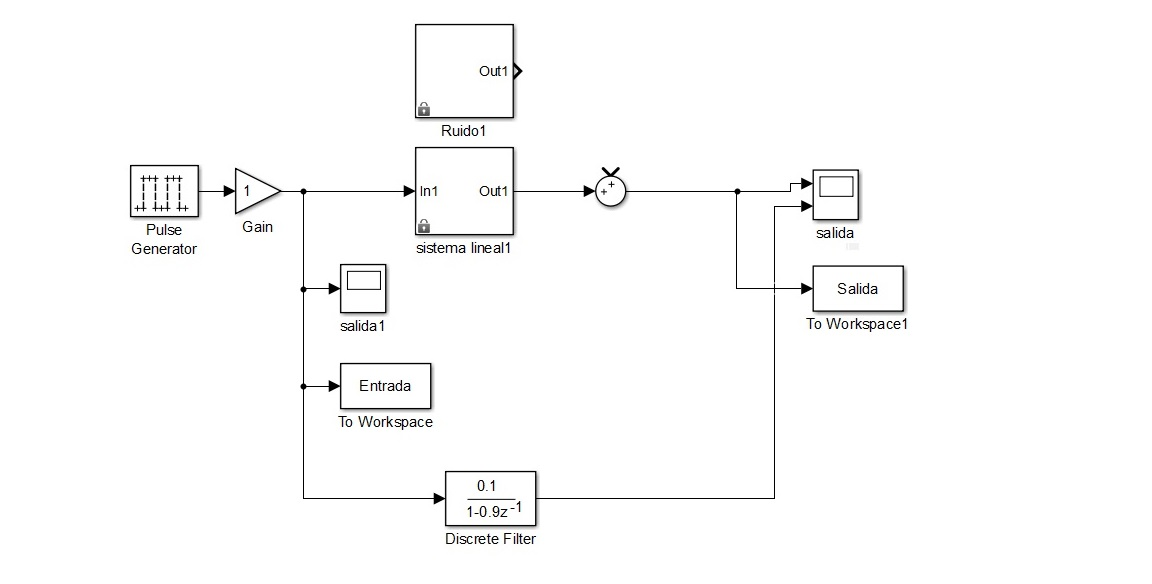
\includegraphics[width=1.0\linewidth]{images/modelFilter.JPG}
		\caption{Modelo Con la función de transferencia identificada}
		\label{Modelo Filtro}
	\end{figure}
	\FloatBarrier
	
	\begin{figure}[h!]
		\centering
		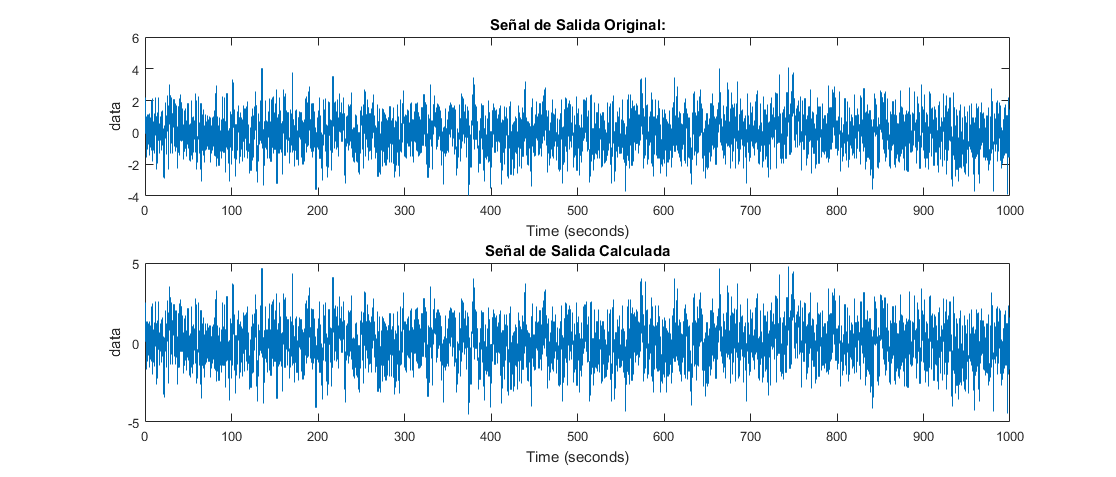
\includegraphics[width=1.0\linewidth]{images/comparative.PNG}
		\caption{Comparativa de las salidas}
		\label{Comparativa}
	\end{figure}
	\FloatBarrier

	Y vemos que ambas salidas encajan exactamente, por lo que \textbf{la función de transferencia queda perfectamente identificada}.
	
	\subsection{Sistema con Ruido}
	
	El sistema con ruido es el original \ref{Modelo Inicial}, para el cálculo de la función de transferencia, hacemos lo siguiente:
	
	\begin{lstlisting}
	>> Zeta = Caract_ZTransform(Entrada.Data,Salida.Data);
	>> theta = Zeta.LeastSquares(1,1)
	
	theta =
	
	-0.8988
	 0.1011
	\end{lstlisting}
	
	Entonces siguiendo la fórmula \ref{Transfer Function}, $-0.8988$ corresponde a $a_1$ y $0.1011$ corresponde a $b_0$, quedando:
	
	\begin{myalign}
		H(z^{-1})= \dfrac{0.1011}{1 - 0.8988z^{-1}}
		\label{TF Noise}
	\end{myalign}
	
	Vemos que es muy parecida a (\ref{TF Identify}), ya que el ruido añadido es pequeño, lo cual podemos ver, si metemos la nueva función de transferencia en simulink.
	
	\begin{figure}[h!]
		\centering
		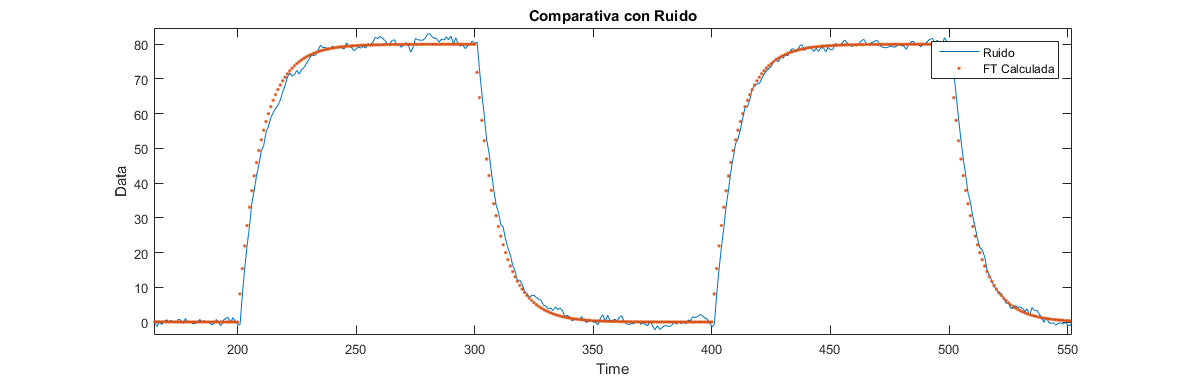
\includegraphics[width=1.0\linewidth]{images/comparative2.PNG}
		\caption{Comparativa de las salidas con Ruido}
		\label{Comparativa2}
	\end{figure}
	\FloatBarrier
	
	Podríamos aumentar el número de polos, pero no mejoraría mucho el encaje entre las dos señales y complicaría la función de transferencia. Por tanto, dejamos identificada la función de transferencia en (\ref{TF Noise}).
	
	\section{Clase \textit{Caract\_ZTransform}}
	
	Adjunto el script con la clase que contiene las funciones anteriormente empleadas:
	
	\lstinputlisting{scripts/Caract_ZTransform.m}
	
\end{document}